% Created 2024-03-20 Wed 14:38
% Intended LaTeX compiler: pdflatex
\documentclass[11pt]{article}
\usepackage[utf8]{inputenc}
\usepackage[T1]{fontenc}
\usepackage{graphicx}
\usepackage{longtable}
\usepackage{wrapfig}
\usepackage{rotating}
\usepackage[normalem]{ulem}
\usepackage{amsmath}
\usepackage{amssymb}
\usepackage{capt-of}
\usepackage{hyperref}
\usepackage{placeins}
\usepackage{gensymb}
\usepackage{hyperref}
\author{Christian Johnson\and\&\and Dan Nusraty\and\&\and Dylan McGill\and\newline Optimail}
\date{\today}
\title{Mail Database Project}
\hypersetup{
 pdfauthor={Christian Johnson\and\&\and Dan Nusraty\and\&\and Dylan McGill\and\newline Optimail},
 pdftitle={Mail Database Project},
 pdfkeywords={},
 pdfsubject={},
 pdfcreator={Emacs 29.2 (Org mode 9.6.15)}, 
 pdflang={English}}
\begin{document}

\maketitle
\newpage
\section*{Preface}
\label{sec:org7461905}
Tasks to complete assignment:
\begin{itemize}
\item Refine application for use
\item Analytics Tracking
\item Reports and Settings Completion
\item Specific classifications/tags for individual packages
\item Secure authorization system for users
\item Logout feature
\end{itemize}


Lessons learned and changes from feedback:
\begin{itemize}
\item Team should focus more on step-by-step procedures, in order to stay organized.
\item Recquire "Admin" or some higher authority credentials to manually add/edit packages within a "database interface"
\item Scanning capability
\item If package is not picked up within 30 days, archive
\item If archived for 6 months, delete from database
\end{itemize}


\section*{Sequence Diagrams}
\label{sec:orgc332bd3}
\subsection*{Dylan - Whole System Overview}
\label{sec:org50d46b9}
\begin{figure}[htbp]
\centering
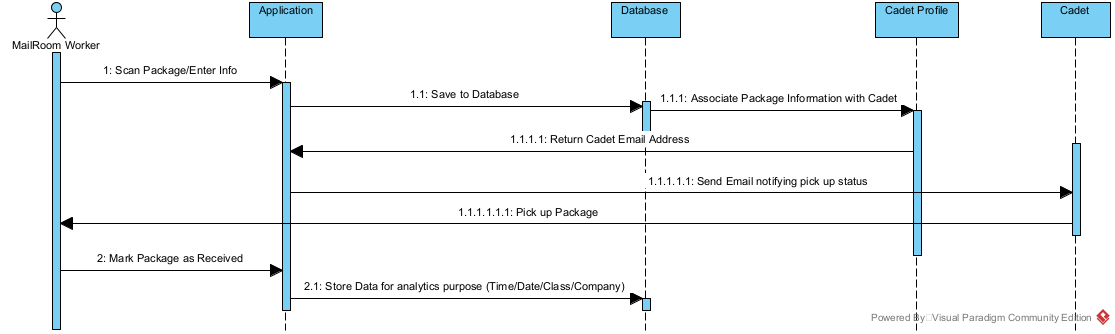
\includegraphics[width=.9\linewidth]{/home/csj7701/Projects/Mail-Database-Project/Class-Documents/SequenceDiagramDylan.png}
\bicaption{---}
\end{figure}

\subsection*{Dan}
\label{sec:orgda4c558}

\subsection*{Christian - "Search Packages"}
\label{sec:org8cbbc42}
\begin{figure}[htbp]
\centering
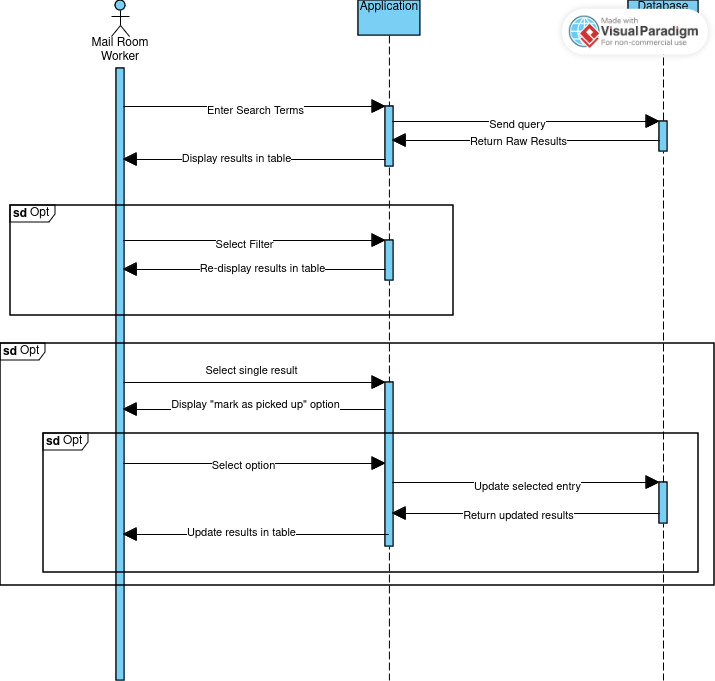
\includegraphics[width=.9\linewidth]{/home/csj7701/Projects/Mail-Database-Project/Class-Documents/SequenceDiagramChristian.jpg}
\bicaption{---}
\end{figure}
\section*{State Diagrams}
\label{sec:org90b4df1}

\subsection*{Dylan}
\label{sec:org24cc351}

\begin{figure}[htbp]
\centering
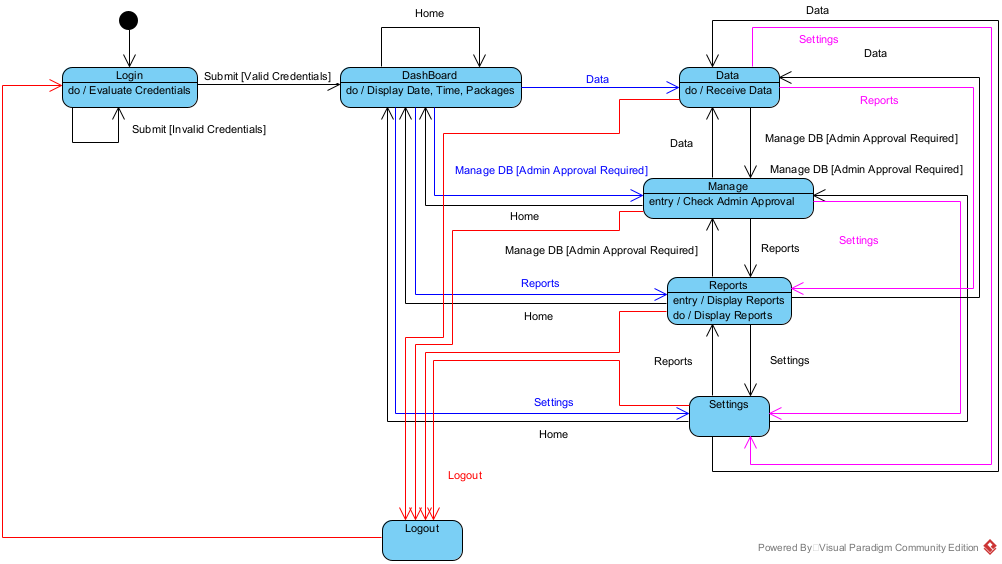
\includegraphics[width=.9\linewidth]{/home/csj7701/Projects/Mail-Database-Project/Class-Documents/StateDiagramDylan.png}
\bicaption{---}
\end{figure}
\subsection*{Dan}
\label{sec:orga24fc5a}

\subsection*{Christian}
\label{sec:orgbc302f8}



\section*{Github Repository}
\label{sec:orgae18b9e}

A \href{https://github.com/CSJ7701/Mail-Database-Project}{Github Repository} has been created. Groupmembers and Instructor were added as collaborators.

\section*{Group Meeting Summaries}
\label{sec:org567001f}

3/6/2024:
\begin{itemize}
\item Reviewed current functionality
\item Reviewed Github functionality
\item Familiarized with Github and Git interfaces
\item Planned for presentation
\end{itemize}


3/8/2024:
\begin{itemize}
\item Planned work assignments
\item Divided work over break
\end{itemize}

3/19/2024:
\begin{itemize}
\item Discussed work done over break
\item Put together Project Part 4 report
\end{itemize}


Activities Reviewed:
\begin{itemize}
\item Reports tab
\item Settings tab
\item Scanner functionality
\item Cadet info/provacy considerations
\item Need to implement logout feature
\end{itemize}

Major decisions:
\begin{itemize}
\item Require admin approval for manage DB option
\item Track company, class, date/time of package pickup (already implemented, need to include in reports)
\item Settings: light/dark mode, ui preferences
\end{itemize}
\end{document}
